\section{Methodology}

\begin{sidewaysfigure}[p]
    \centering
    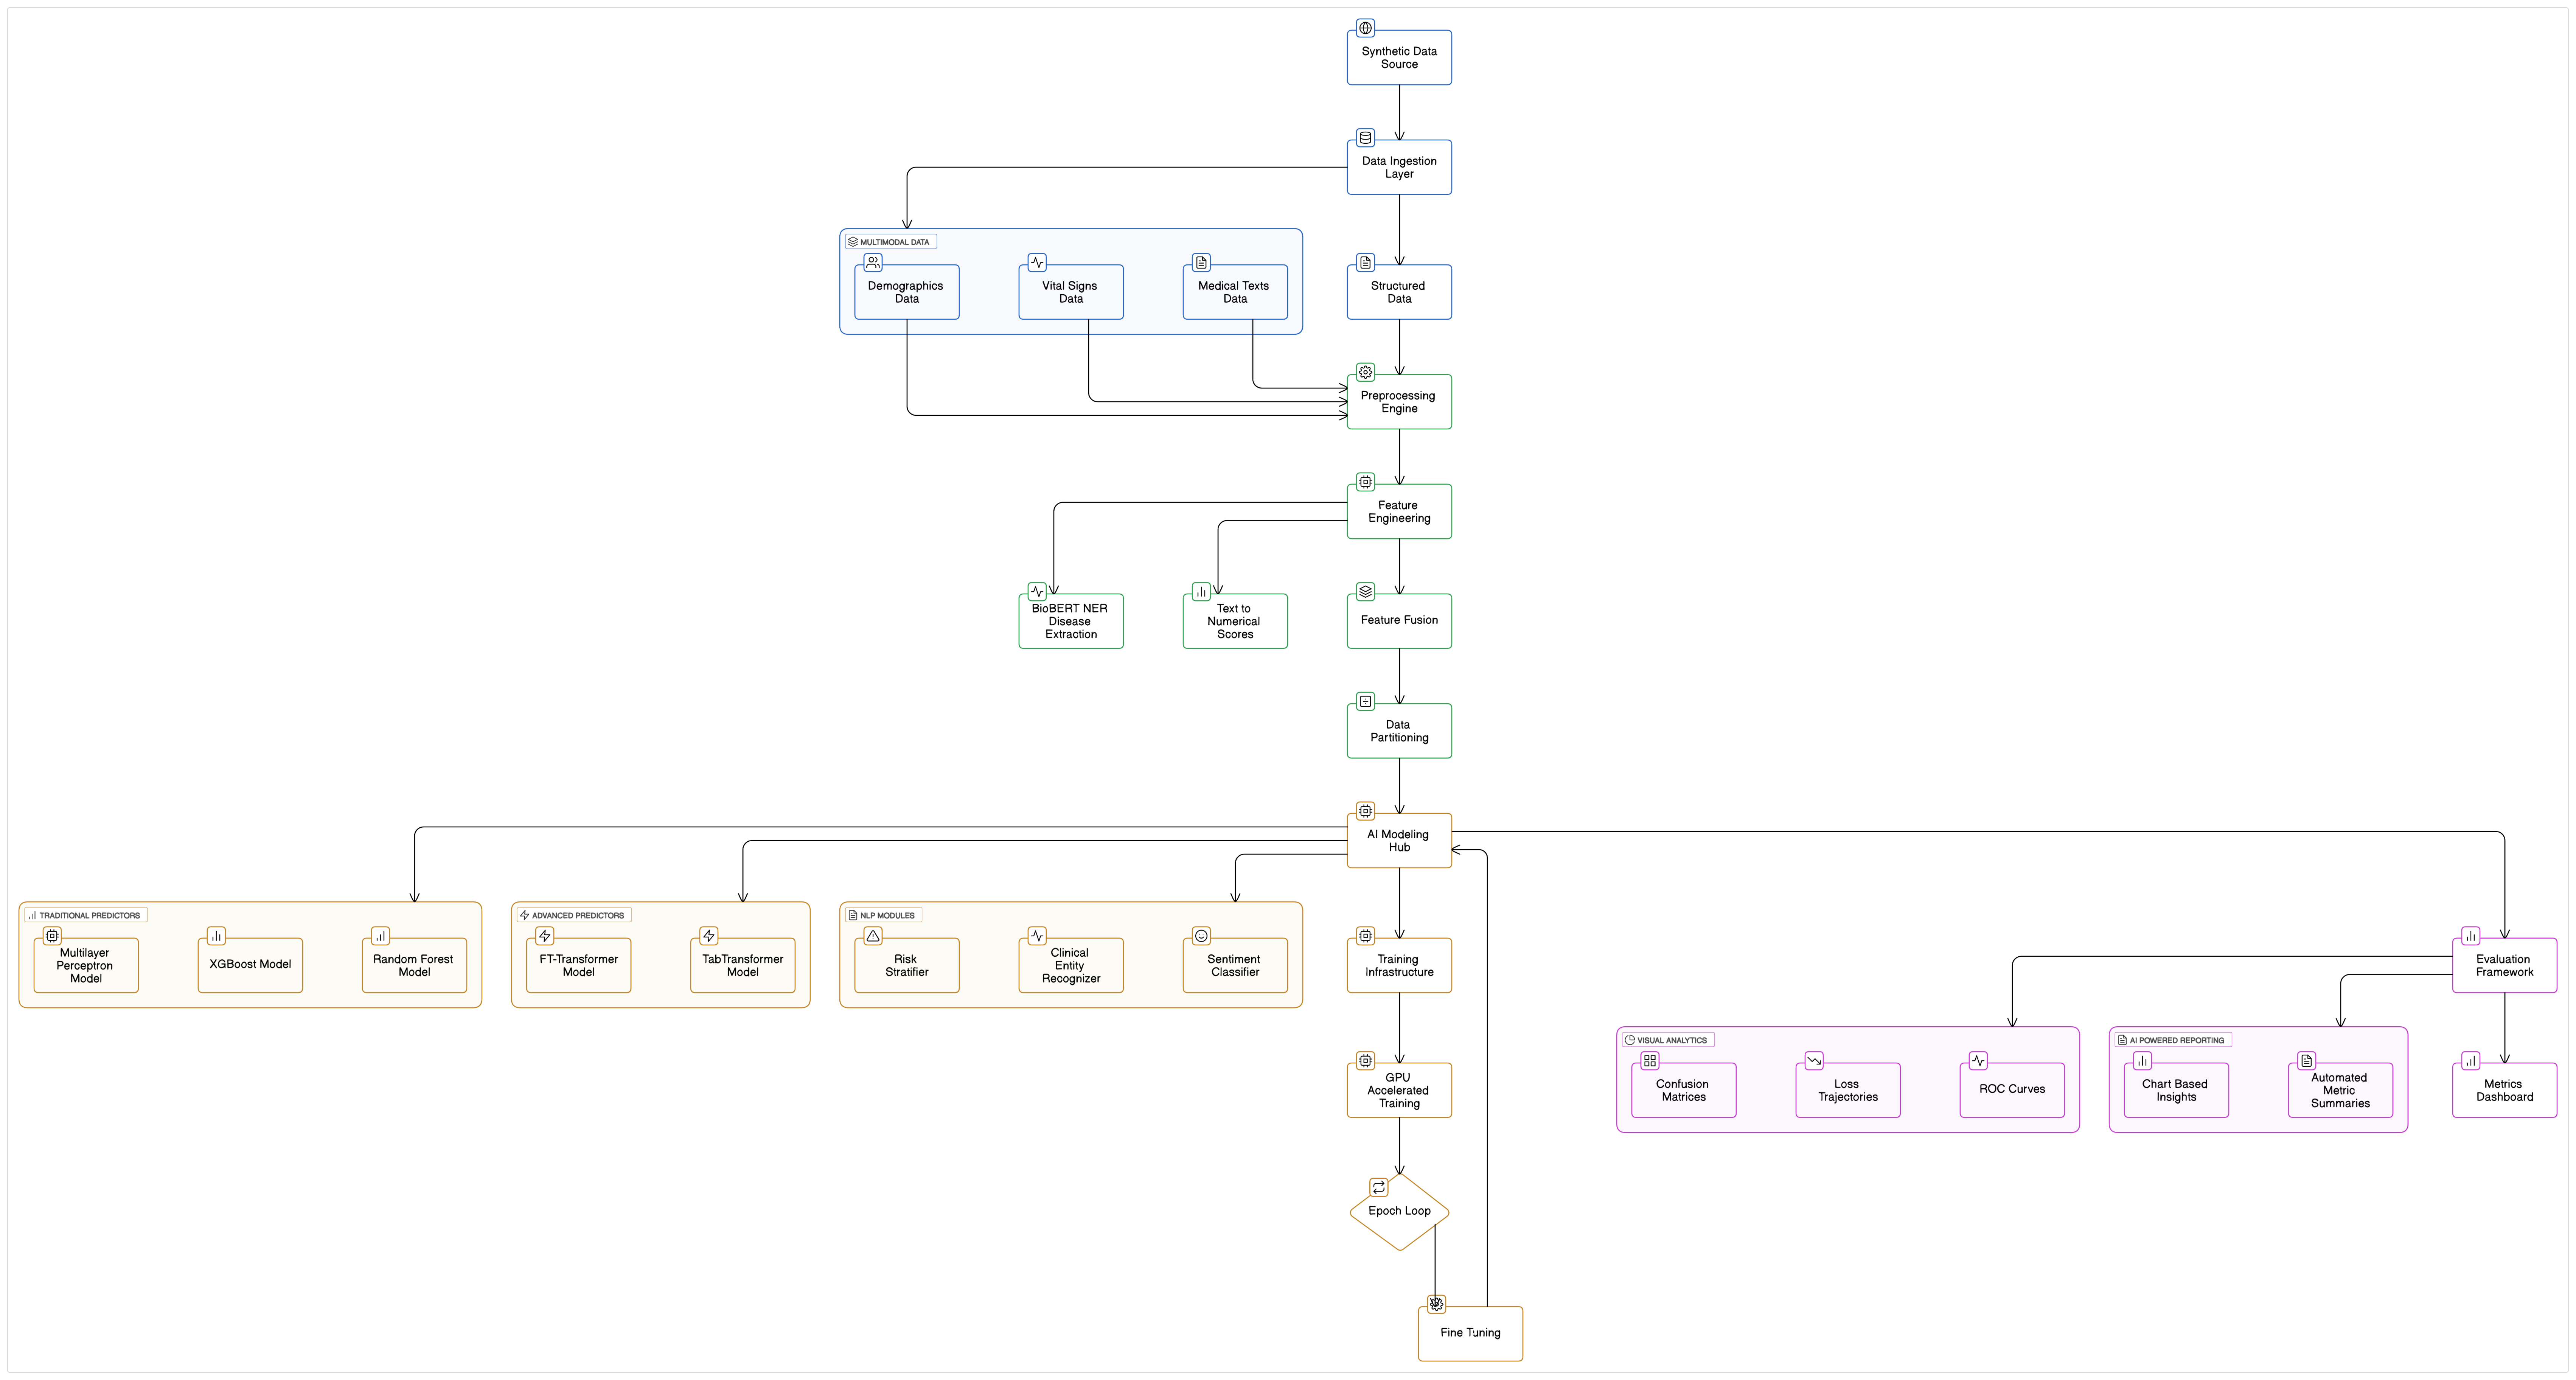
\includegraphics[width=0.8\textwidth]{../images/architecture.png} % Replace with your image path
    \caption{Project Architecture Overview}
    \label{fig:project_architecture}
\end{sidewaysfigure}

This study's methodology commenced with dataset simulation and feature engineering, where synthetic patient data was generated using \textit{Gemini 2.5 Flash-Preview-0417} \parencite{Doshi_2025} in JSON format, encompassing fields like \texttt{patient\_id}, demographics, \texttt{textual medical\_history}, \texttt{vital signs}, and questionnaire responses (e.g., \texttt{describe\_fatigue\_level}, \texttt{describe\_lifestyle}, \texttt{describe\_mental\_health}); this approach addressed challenges related to data privacy, availability, and enabled controlled scenario generation. Feature engineering involved Named Entity Recognition (NER) from \texttt{medical\_history} using BioBERT \parencite{Lee_2019} to extract disease entities, and the quantification of textual questionnaire responses into a 1-5 numerical severity scale by \textit{Gemini 2.5 Flash-Preview-0417}, converting subjective data into structured, machine-learning-compatible features. The final feature set integrated these engineered elements with numerical vital signs and categorical demographics. Subsequently, predictive model development focused on patient deterioration classification, employing a binary \texttt{deterioration\_label} and evaluating traditional machine learning models (\textit{Random Forest, XGBoost, MLP}) alongside transformer-based tabular models (\textit{TabTransformer} \parencite{huang2020tabtransformertabulardatamodeling}, \textit{FT Transformer} \parencite{gorishniy2023revisitingdeeplearningmodels}), trained for up to 30 epochs with standard data splits. Specialized NLP tasks were also undertaken: sentiment analysis on \texttt{describe\_lifestyle} using \textit{Google BERT-Large} \parencite{devlin2019bertpretrainingdeepbidirectional}; clinical text interpretation (NER with IOB tagging) on \texttt{medical\_history} via a fine-tuned \textit{Bio-Clinical BERT} \parencite{ling2023bioclinicalbertbertbase}; and risk classification for \texttt{describe\_fatigue\_level} and \texttt{describe\_mental\_health} using separate fine-tuned BERT base models, with these NLP model trainings conducted on A100 GPUs via Google Colab. Model evaluation and interpretation utilized metrics such as Accuracy, Precision, Recall, F1-score, and ROC-AUC, justified by their comprehensive assessment capabilities and the critical importance of recall in health contexts, complemented by visualizations including ROC curves, training loss curves, and confusion matrices. AI-assisted interpretation, leveraging \textit{Gemini 2.5 Flash-Thinking-Preview-0417} for analyzing metrics and figures, was guided by prompts engineered with \textit{Grok 3} \parencite{xGrokBeta} and \textit{Gemini 2.5 Flash-Thinking-Preview-0520}. The overall research was implemented in Python, utilizing key libraries such as \texttt{Scikit-learn, Pytorch, Hugging Face Transformers, XGBoost, Pandas, NumPy, Matplotlib}, and \texttt{Seaborn}, within a Jupyter Notebook environment on the Google Collab platform and local setup.